\documentclass{memoir}

% need it in .docx form? no problem!
% pandoc -s chapter-1.tex -o chapter-1.docx --bibliography="chapter-1.bib"; mv chapter-1.docx ~/Desktop

\usepackage{import}
\import{../}{gov-style}
% \addbibresource{../thesis.bib}

\begin{document}
\begin{refsegment}
\epigraph{``Spying on people by magic is the same as spying on them in any other way.''}{---\textup{C.S. Lewis}, The Voyage of the Dawn Treader}

\section{The OPM hack}
\subsection{You know every place I've lived since I was 18}
One morning in April 2015, while performing a routine security check, a man named Brendan Saulsbury identified an odd bit of outbound network traffic. Saulsbury worked as a cybersecurity engineer for the United States Office of Personnel Management (OPM), functionally the human resources department for the federal government. Saulbury noticed that, from somewhere within OPM, a computer was sending brief updates to a website registered at opmsecurity.org---a domain address designed to look like an official system, but not actually belonging to the US Government or the OPM security team. He alerted Curtis Mejeurm, one of OPM's senior IT strategists, and it quickly became clear that this small beacon was the surface marker of an iceberg. The US Computer Emergency Readiness Team set up shop the next day in an adjacent basement room and hunkered down to investigate and destroy the malware. 10 days, 2000 items of malware, and 1 scheduled power outage later, government security engineers declared that to the best of their knowledge the threat had been removed.\footcite{koerner_inside_2016} But the work to identify the scope of the damage had only just begun.

US officials would only confirm that they believed a ``foreign entity or government'' had been behind the attack, but it was an open secret that they suspected the involvement of the Chinese government.\footcite{spetalnick_china_2015} Internal investigators determined that the department had been the victim of an attack perpetrated by an advanced persistent threat (APT), a formally organized and typically state-sponsored group of hackers.\footcite[Attributing a cyberattack is difficult because hackers have endless means to obscure their orgins. In this case, however, the first clue that investigators found was left there on purpose. A particularly effective group of hackers tied to China has made it a calling card of sorts to register sites using the names of members of Marvel's comic book superhero group, The Avengers. In this case, opmsecurity.org was registered under the name ``Steve Rogers,'' better known as Captain America.]{koerner_inside_2016} They began to put together a damage report. From preliminary estimates, it appeared that perpetrators had stolen the identifying information of up to 4 million current and former federal employees, including personal finances and fingerprint data. The hackers had been present in the system for at least half a year.

As investigations continued, the news got worse; the scope of the attack greatly exceeded the initial estimates. The Chinese had accessed an OPM database of applications for security clearance which exposed not just the personal data of the applicants themselves but also the detailed information they had supplied about their family and friends.\footcite{nakashima_hacks_2015} Millions of social security numbers, job applications, and home addresses had been compromised, including information about personnel at the highest levels of government. When the government announced the the full extent of the damage, it caused an uproar. The American Federation of Government Employees, the largest federal workers union, filed a class-action lawsuit against OPM, seeking damages under the Privacy Act.\footcite[The lawsuits were later dismissed.]{chalfant_court_2017} Mark Warner (D-Va.), a member of the Senate Intelligence Committee whose constituents included many of the employees affected, called for OPM Director Katherine Archuleta's resignation. Because the information might be used for identity theft, the US government preemptively offered all affected employees free credit and identity monitoring services for three years.\footcite{nakashima_hacks_2015}

Not only was the OPM hack a public relations disaster, it had enormous implications for national security and counterintelligence. US officials feared that the stolen records could expose undercover CIA operatives working in embassies around the world, whose names would be suspiciously absent from the OPM records.\footcite{nakashima_hacks_2015} The information could be used by a foreign intelligence service to identify American officials who might be susceptible to pressure, or worse, recruitment. FBI Director James Comey personally took questions about the incident. ``If you have my [application for security clearance],'' Comey said, ``you know every place I've lived since I was 18, contact people at those addresses, neighbors at those addresses, all of my family, every place I've traveled outside the United States. Just imagine if you were a foreign intelligence service and you had that data.''\footcite{nakashima_hacks_2015} Now the Chinese intelligence service did and, more disturbingly, there were no signs of what they intended to do with it.\footcite{koerner_inside_2016}

\subsection{You don't do that stuff secretly}
The White House immediately took steps to minimize the possibility that a data breach of that scale would ever happen again. It launched a Cybersecurity Sprint that pushed the heads of federal agencies to speed up adoption of security best practices, like updating software and enabling two-factor authentication.\footcite{koerner_inside_2016} A few months later, the White House announced the Cybersecurity National Action Plan (CNAP), proposing a \$3.1 billion Information Technology Modernization Fund, a \$19 billion allocation for cybersecurity deficiencies, and a National Cybersecurity Alliance that would partner with leading technology and finance companies to secure the accounts of private citizens.\footcite{the_white_house_fact_2016} These were laudable and necessary measures, but they focused entirely on defending against future cyberattacks without addressing what caused the attack in the first place. The omission was deliberate---in responding to the OPM hack, the United States chose not to punish the perpetrators.

Consider what the OPM hack represented diplomatically. An advanced group of hackers conclusively linked to the Chinese military had conducted a months-long operation to infiltrate secure federal computer systems. The data stolen from OPM was so consequential that its director was forced to resign. In response, the White House launched a nation-wide cybersecurity initiative, but failed to acknowledge that the impetus for the initiative was a cyber-attack by an often-adversarial foreign nation. The Obama administration did not announce a single action that could be interpreted as a retaliatory measure against the Chinese government for stealing the personally identifying information of 21 million Americans. The Chinese got away with it.

Plenty of conditions can alter how one state responds to an aggressive act by another---especially when those states have as complicated a relationship as the US and China do---but for an attack of that magnitude to pass without response struck many as remarkably strange. ABC News reporter Jonathan Karl was one such person, and he raised the issue in a press briefing just before President Obama left office. This briefing took place right after the United States had issued a series of sanctions against the Russian Federation for its cyber-enabled interference in the 2016 US Presidential Election. In the exchange below, Karl asked Press Secretary Josh Earnest how the White House could justify responding so harshly to the Russians when it had completely let the Chinese off the hook (emphasis mine):\footcite[You can watch the full exchange via video here. It's pretty awkward.]{gill_earnest_2017}

\begin{quote}
KARL: \textbf{So when the Chinese hacked OPM in 2015 [...] why did the White House do nothing publicly in reaction to that hack}, which, in some ways, was even more widespread than what we saw here from the Russians, allegedly?
\newline \newline
EARNEST: Well, I think that what we've seen is that these are two cyber incidents that are malicious in nature, but materially different.
\newline \newline
KARL: Twenty-one million people had their personal data taken.  \textbf{Fingerprints, social security numbers, background checks -- I mean, this was a far-reaching hack.}
\newline \newline
EARNEST: \textbf{I'm not downplaying the significance of it, I'm just saying that it's different} than seeking to interfere in the conduct of a U.S. national election. I can't speak to the steps that have been taken by the United States in response to that Chinese malicious cyber activity.\footcite[Transcript adapted from the official White House website.]{earnest_press_2017}
\end{quote}
But... why? What about electoral interference demands a material sanction from the US Government that is not true of cataclysmic data theft? Earnest did have a good answer for this question, and given the political significance of the issue, he absolutely should have. Karl correctly observed that the OPM hack was more directly invasive than anything the Russians did in 2016. Hacking sensitive government networks is probably more of an affront to national security than buying divisive Facebook advertisements; from a legal perspective, the Chinese case is a more clear-cut violation of international law.\footcite[p.~625]{terry_dont_2018} Karl pressed Earnest on this question, listing a number of actions that would be reasonable, proportional responses to the situation, and confirming that the US government elected to pursue none of them.

\begin{quote}
KARL: But nothing was announced. There was not a single step announced by the White House in response to that.
\newline \newline
EARNEST: That is true that there was no public announcement about our response, but I can't speak to what response may have been initiated in private.
\newline \newline
KARL: \textbf{But no diplomats expelled, no compounds shut down, no sanctions imposed, correct?}
\newline \newline
EARNEST: Well, again, I can't speak to --
\newline \newline
KARL: \textbf{You don't do that stuff secretly.}  I mean, that's --
\newline \newline
EARNEST: Well, certainly when it comes to the diplomats, that's right, there were no diplomats PNGed. That's something that we would announce publicly.
\end{quote}
Not only can you not do ``that stuff'' secretly, establishing norms and deterring future malicious behavior would seem to require that you do it as publicly as possible. The White House even acknowledged that they needed to be more public in their response for the purposes of deterring attacks like the OPM hack.\footcite{sanger_u.s._2016} Supposedly, it considered covert cyber-retaliation measures as well as punitive economic sanctions, though the latter of never materialized and there is no publicly-available evidence of the former.\footcite{nakashima_hacks_2015} Obama administration officials refused until the very end to officially name China as the culprit. The first time a US government official formally attributed the OPM hack to the Chinese government was in September 2018.\footcite{sanger_trump_2018} By then the window for a comeback response was long gone.

\subsection{You have to kind of salute the Chinese for what they did}
There is a substantive difference between OPM hack and the Russian electoral interference, but it is one that politicians have a difficult time acknowledging. From the perspective of senior policymakers, the OPM hack looks a lot like the traditional practice of espionage---foreign operatives accessing a classified database and collecting information about US officials.\footcite{nakashima_chinese_2015} An adversarial intelligence service transmitting sensitive government records is a type of threat that the counterintelligence community has seen before. The opmsecurity.org was functionally a digital spy.

When a cyberattack is characterized as traditional espionage, it limits how strongly the federal government will respond. The Congressional Research Service (CRS) report about the OPM hack quoted an unnamed Senior Administration Official, who said that the White House had been clear ``that there is a vast distinction between intelligence-gathering activities that all countries do and the theft of intellectual property for the benefit of businesses in the country, which we don't do and we don't think any country should do.'' The not-at-all subtle implication was that espionage for other purposes \emph{is} something that we do, and don't necessarily think other countries should refrain from doing either. The CRS report concluded that the OPM breach ``appears to be seen in the category of intelligence-gathering,'' for which counterintelligence, not prosecutions, is deemed to be the appropriate response.\footcite{finklea_cyber_2015}

While discussing the OPM hack, a few high-ranking public officials simply admitted that spying on political and military institutions is an accepted component of statecraft. Ranking House Intelligence Committee member Adam Schiff (D-Calif.) spoke with surprising candor when he said ``I think we have to be careful about the importance of continuing to draw a line between theft for economic advantage and traditional foreign intelligence activities, which may look untraditional now that they’re in the cyber realm.''\footcite{nakashima_hacks_2015} John Brennan, Director of the CIA, described foreign spying on domestic political institutions as ``fair game.''\footcite{sanger_u.s._2016} And while speaking at an intelligence conference, James Clapper, Director of National Intelligence, committed a classic Kinsley gaffe---saying what every official knows to be true but would never admit out loud: ``You have to kind of salute the Chinese for what they did. If we had the opportunity to do that, I don't think we'd hesitate for a minute.''\footcite{pepitone_clapper_2015} When pressed, he declined to repeat the comment, but, to the best of my knowledge, he never disavowed it.\footcite{sanger_u.s._2015}

There have been a number of high-profile cyberattacks in recent years, but the OPM hack best illustrates the question that motivates this thesis: why does the United States consider cyberattacks with traditional intelligence purposes to be relatively immune from diplomatic recourse? The comments of senior officials suggest the answer to that question has little to do with cyber policy itself. The American response to cyberattacks is often muted because in cases where the attack the response is informed by the already-established norms of peacetime espionage. Rep. Schiff suggests that policymakers are interested in porting those norms to cyber policy; I want to know whether they should.

In the remainder of the introduction, I will conduct a brief review of US cyber policy---establishing that the United States' response to cyber espionage is inconsistent with its stated cyber policy and that the discrepancy can only explained using the historical norms of espionage. The next section will argue that both domestic cyber law and the national cybersecurity strategy are inadequate frameworks to explain American policy response. The section after shows that the United States will never respond to cyberattack with punitive measures if it believes that that the attack constitutes traditional espionage---even when the damage done by that espionage is significant. In the final section section, I will conduct a literature review to demonstrate the missing application of espionage norms to cyber policy, and I will outline a research design to define exactly what espionage norms are, where they come from, and how they apply to cyber policy today.

\section{The hole in US cyber policy}
\subsection{Developing international norms through domestic law}
In order to understand how espionage norms influence United States cyber policy, it is important to first understand the hole in the legal framework that espionage helps to fill. Absent comprehensive, enforceable treaties, there is no separate set of laws that guide the prosecution of domestic and international cyber crimes---there are only the domestic laws, with which the US can prosecute domestic criminals or foreign nationals in friendly territory.\footnote{There are, of course, \emph{some} treaties that deal with international cyber law. They are however few and far between, and with the possible exception of the Budapest Convention, mostly irrelevant to the decision-making of major actors today.} Enforcing domestic law is one of the most promising ways for new international norms to form.\footcite[p.~295]{deeks_international_2015} If the US has a robust legal regime regarding cyberattacks, it can use that to pressure countries who choose to attack it.

The problem with building cyber norms from domestic law is that government is often slow to adapt. Domestic laws that criminalize hacking federal computers are very new and applying them to any issues of geopolitical significance is even newer. The first time the federal government addressed the issue was in a 1977 General Accounting Office (GAO) report entitled ``Security of Computer Systems.''\footcite{washington_post_staff_timeline_2003} In the report and resulting testimony, GAO director Donald Scantlebury warned Congress about the threat of a ``computer burglar.''\footcite{u.s._government_accounting_office_security_1977} It took Congress an additional seven years to pass the first federal computer crime legislation.\footcite[The later bill cited here, the Computer Security Act of 1987, describes the 1984 bill as being the first federal legislation in this area.]{glickman_computer_1988} The ``Counterfeit Access Device and Computer Fraud and Abuse Act of 1984'' made it a federal offense to produce a ``fraudulent access device.''\footcite{hughes_access_1984} Around this time, the government built an internal tool that someone might want to access fraudulently---an internet precursor called ARPAnet---and four years later, a Cornell graduate student would do exactly that.

Robert Morris created the first computer worm (a type of virus) by accident. The program, which came to be known as the Morris Worm, was supposed to demonstrate the weakness of federal network security by accessing as many computers as it could. Instead, the virus self-replicated with unexpected velocity and crashed thousands of ARPAnet computers over the course of a few days in November 1988 before it was finally contained.\footcite[This source, a master's thesis for the USAF Air University, makes the dramatic and completely unsubstantiated claim that the Morris worm infected half of of ARPAnet's 88,000 computers. The more popular (and plausible) claim is that of the roughly 60,000 ARPAnet-connected computers, the worm infected 10\% of them, though that number is not particularly well substantiated either.]{moore_conception_2014} Even though Morris was one of the first felony convictions under the Computer Fraud and Abuse Act, a GAO report requested by Congress noted that cases like these were still somewhat difficult to prosecute due to the lack of federal statutes directed at computer-virus-type incidents, and the government began to take cybersecurity more seriously.\footcite{u._s._government_accounting_office_computer_1989} The Morris Worm permanently altered the public perception of the internet, which until then had felt ``like a small town where people thought little of leaving their doors unlocked.''\footcite{lee_how_2013}

It was not until the Clinton administration that the federal government properly addressed the need to keep the doors locked---to both domestic threats and foreign ones. CIA Director John Deutch testified to the Senate in 1996 that ``hackers, criminal groups, and foreign intelligence services consider [information systems] lucrative targets,'' noting that a handful of foreign nations have already instituted ``formal information warfare programs.''\footcite{deutch_worldwide_1996} That same year, Executive Order 13010 created the President's Commission on Critical Infrastructure Protection, designed to protect ``critical infrastructures from physical and cyberthreats and assuring their continued operation,'' covering utilities like water, power, fuel, telecommunications, and financial services.\footcite[~p.761]{boys_clinton_2018} The inclusion of cyberthreats alongside physical ones signified a landmark understanding of the actual threat that the internet posed---not just as a new system of infrastructure to defend, but as a vector by which all legacy infrastructure was soon to be made vulnerable as well.

1996 marked the first year that the United States first recognized that foreign agents might try compromise its computer systems and maintained a domestic legal regime in order to prosecute those who try. The time between the first warnings of a ``computer burglar'' and the recognition of other states' ``formal information warfare programs'' spanned 20 years, roughly the same amount of time between 1996 and today. For much of the time since, the lack of protests regarding cyberattacks, especially from nations who have suffered aggressive forms of them, has been remarkable.\footcite[p.~132]{brown_customary_2012} Chinese espionage and Russian interference have lately made it impossible for the United States to dodge the question of diplomatic response, but until the last few years, the customary practice of states was to diplomatically ignore most cyber activity that fell below the use of force.\footcite[p.~141]{brown_customary_2012} The US has laws against cyber espionage---no state can argue that cyber intrusions are somehow legally undefined---but it has been reluctant to use them in such a way that would encourage a norm to develop against it. Only recently has the US begun to charge foreign nationals under domestic law for cyber crimes.

\subsection{Existing diplomatic enforcement mechanisms}
Domestic laws are not the only way to set a norm about the use of state power in cyberspace---a national cybersecurity strategy that explicitly addresses how the US will respond to foreign attacks could guide state practice as well. Starting with Bill Clinton, each American president has put out a document detailing their cyber strategy.\footnote{In order: ``The National Plan for Information Systems Protection'' (Clinton), ``National Strategy to Secure Cyberspace'' (Bush), ``International Strategy for Cyberspace: Prosperity, Security, and Openness in a Networked World'' (Obama), ``National Cyber Strategy of the United States of America'' (Trump). The Trump strategy document claims that it is the ``first fully articulated cyber strategy in 15 years.'' It does not specify whether it simply ignored the Obama-era strategy document or if it doesn't consider that strategy to be a ``fully articulated cyber strategy,'' but the statement is in either case incorrect.} These plans are always incredibly vague on the subject of how the United States will respond to a cyberattack by a foreign power. The Bush strategy, for instance, was criticized at the time for its lack of enforcement mechanisms.\footcite{lemos_bush_2003} President Obama introduced a number of official directives dealing with cybersecurity, but for most of his presidency these generally lacked enforcement mechanisms as well. Assessing Obama's efforts to secure the nation against cyberthreats in 2013, PolitiFact outlined the various features of his cyber strategy and its associated directives, then bluntly noted: ``So that's what has happened. What hasn't happened: a change in law.'' The editors gave his promise to ``develop a comprehensive cybersecurity and response strategy'' a grade of ``In the Works.''\footcite{moorhead_work_2013}

% Late in its tenure, the Obama administration took some actions that shifted the focus of cybersecurity policy from prevention and defense to mitigation and response---a shift that the Trump administration has since embraced. Just as the military would never say that its "missiles strategy" was to not get hit by missiles, so too was it time to stop saying that our cybersecurity strategy was to secure our nation against cyberattacks.

To the extent that the United States has a comprehensive cyber strategy---with an associated set of enforcement mechanisms---it is a collection of structures set up towards the end of the Obama administration and modified during the Trump administration. There are two Obama-era actions in particular that directly address American response to cyberattacks originating from a foreign power. The first is Presidential Policy Directive 41, which codifies varying degrees of severity for a given cyber incident (Figure \ref{severity-schema}) and sets the principles that guide its response. The other is Executive Order 13694, which authorizes the Secretary of the Treasury ``to impose sanctions on those individuals and entities that he determines to be responsible for or complicit in malicious cyber-enabled activities that are reasonably likely to result in, or have materially contributed to, a significant threat to the national security, foreign policy, economic health, or financial stability'' of the US, and it was later amended to include election interference as well.\footcite{daniel_our_2015} Not only did the Trump administration leave the order in place, it quietly extended the order in 2017.\footcite{uchill_white_2017}

\begin{figure}
\centering
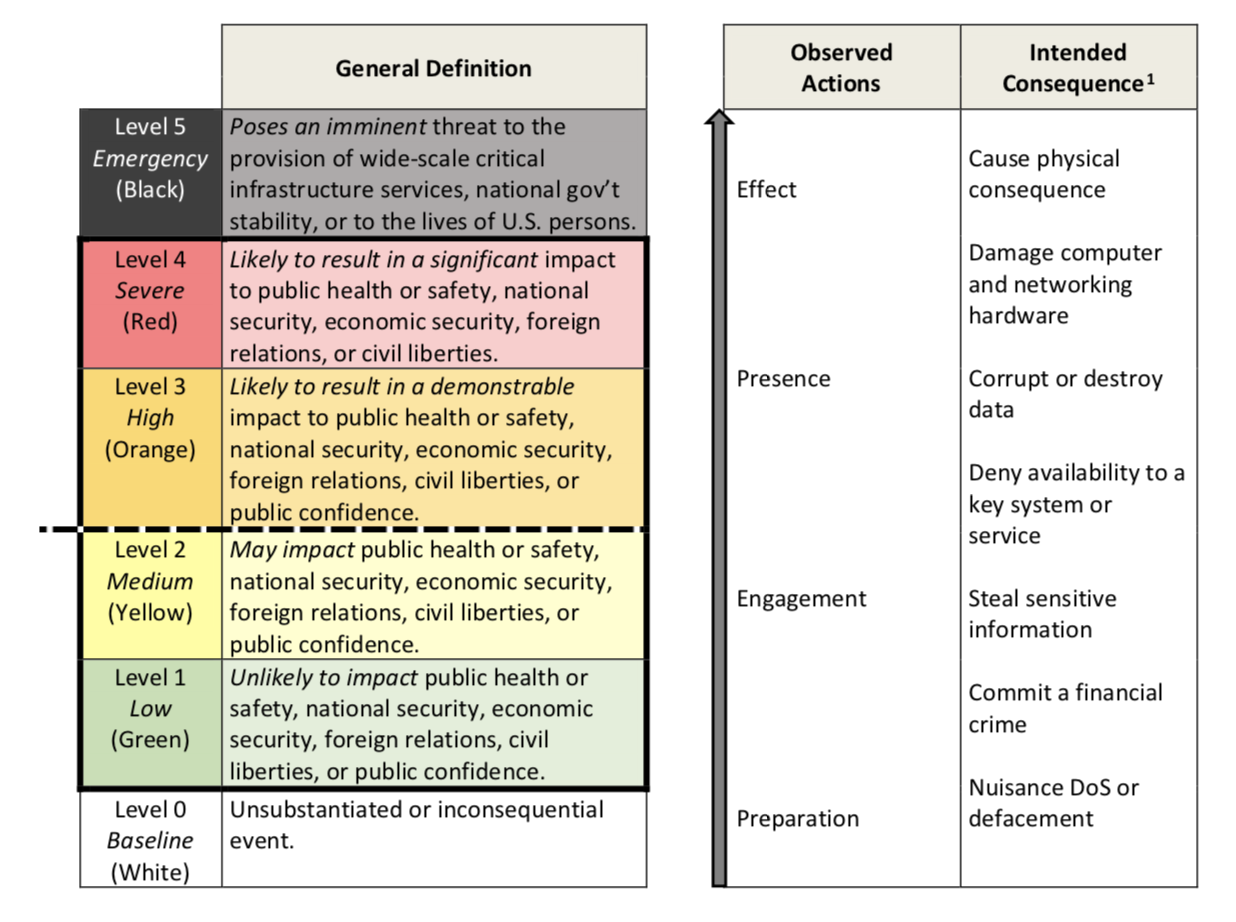
\includegraphics[scale=0.53]{severity-schema.png}
\caption{Cyber Incident Security Schema}
\label{severity-schema}
\end{figure}

Despite the controversy surrounding Russian interference in the 2016 election---and President Trump's subsequent reluctance to address or attribute it---so far there really hasn't been much daylight between his administration's stated strategy on cybersecurity and that of the administration prior. Though more martial and aggressively worded as per his style, Trump's 2018 cybersecurity strategy offers few specifics that contradict any Obama-era strategy. Christopher Painter, former White House Senior Director for Cyber Policy, argues that it ``sends a strong message of continuity to our public and our partners.''\footcite[Painter also served at the State Department for six years as the Coordinator for Cyber Issues, which at the time was an Assistant Secretary level position. Since then, its status within the department has fluctuated wildly. Rex Tillerson, Trump's first Secretary of State, announced that he would abolish the office and merge it into State's Bureau of Economic Affairs. Then, just a few months later, he proposed creating an entirely new department bureau with a Senate-confirmed Assistant Secretary, possibly in response to criticism of his first decision. Though current Secretary Mike Pompeo appears to have more interest in cyber policy, the State Department still has not reestablished a high level cyber position.]{painter_white_2018} Part of the continuity is because a lot of Obama's achievements in the cyber realm were heavily technocratic, and the Trump administration ``National Cyber Strategy of the United States of America'' is light on specifics to contradict them.\footcite{guest_blogger_white_2018} Towards the end of his presidency, Obama signed measures to promote public-private information sharing, secure financial transactions, and establish the Cyber Threat Intelligence Integration Center.\footcite[Among other actions taken during the Obama presidency, these were sufficenct for PolitiFact to update its 2013 rating of his cyber-enforcement actions to ``Promise Kept.'']{carroll_obama_2016} Most of these measures are still in effect, and as far as we know continue to guide our cyberattack response.

The one area in which the Trump administration has pointedly diverged from Obama-era cyber policy is in constraints on the offensive use of cyberattacks. In August 2018, President Trump signed a classified order rescinding Obama's Presidential Policy Directive 20, which had the practical effect of ``delegating authority to the defense secretary to use cyber tools and techniques to disrupt or degrade an adversary's network or choke off attacks underway''\footcite{nakashima_trump_2018} Previously, such an attack would have to have been vetted by the State Department and intelligence agencies, which some within the Department of Defense (DoD) and Cyber Command found limiting.

Rescinding PPD-20 constitutes a significant step by the Trump administration to reduce the constraints on US Cyberwarfare operations. The Obama administration had been reluctant to do so, worried that giving more authority to the military to authorize offensive operations increased the risk that other concerns (diplomatic, legal, economic) might not get weighted equally.\footcite{starks_ramifications_2018} The end of PPD-20 also reduces some of the incentive to cooperate with civilian intelligence services, making it more likely that the military decides to operate without sufficient information, potentially even compromising an existing operation run by a civilian agency.\footcite{hawkins_cybersecurity_2018} General Paul Nakasone, director of both the National Security Agency and the United States Cyber Command, and the person with whom the authority to launch a cyberattack now rests, expressed frustration during his Senate confirmation hearing that America's adversaries attacked us online with little concern for retaliation.\footcite{sanger_trump_2018}

When it is interested in doing so, the United States does not lack for options to respond to a cyberattack. The Department of the Treasury can unilaterally impose sanctions on entities suspected of cyber activities that endanger ``national security,'' a broad term that leaves the office with a lot of discretion. By removing PPD-80, the Trump administration made it appreciably easier for the military to engage in offensive cyberattacks, which should theoretically be a deterrent. And of course policymakers still have access to other, more traditional deterrent tools. In response to a damaging cyberattack, the US could expel diplomats from the offending nation, impose financial sanctions on a relevant portion of their economy, or refuse to cooperate on other diplomatic issues until certain conditions are met. Theoretically, it could even threaten military retaliation for a cyber intrusion.

\section{The intelligence exception}
\subsection{Designating cyberattacks as espionage}
The United States federal government, its intelligence agencies, and its military have significant leeway to penalize states and state-sponsored entities for malicious cyber-activities---and they often choose not to. Presidential administrations have spent the past 20 years issuing documents that stress the need to expand our cyber defenses, and the past 5 years issuing documents that promise the United States will respond appropriately to a cyberattack that is ``likely to result in demonstrable harm to the national security interests, foreign relations, or economy of the United States or to the public confidence, civil liberties, or public health and safety of the American people.''\footcite{office_of_the_press_secretary_fact_2016} They only use them, however, when a cyberattack cannot be characterized as political or military espionage.

% One common excuse you hear from spokespeople is that attributing cyberattacks is difficult, so their retaliatory options are limited by uncertainty. Yes, definitively attributing cyberattacks is difficult, but there is also no external standard of proof that intelligence agencies have to meet in order to justify a response---the relevant policymakers just have to be convinced that the intelligence justifies their actions. That's how we ended up in Iraq. In the case of the OPM hack, investigators were sure from almost the very beginning that the parties responsible were affiliated with the Chinese government. Once the government has determined the origin and the nature of the harm with a sufficient level of certainty, it then falls on the policymakers to determine a response, and that is where the guidelines that the US government publishes cease to have any explanatory power.

Compare the government response to the OPM hack with the fallout from the Sony hack of 2014. Hackers affiliated with the North Korean government stole sensitive information and leaked damaging emails from Sony executives, supposedly in retaliation for the upcoming James Franco/Seth Rogen comedy about assassinating North Korean leader Kim Jong-Un.\footcite{barnes_sony_2017} The government responded swiftly; the Sony hack was the first time a sitting US president publicly accused a foreign nation of launching a cyberattack and promised retaliation.\footcite{sanger_u.s._2016} The US made good on its threat, and direct sanctions were imposed on North Korea the following year.\footcite{lederman_us_2015} A Washington Post article called the response ``unprecedented,'' which compared to how the US had previously responded to cyber espionage, it absolutely was.\footcite{nakashima_why_2015}

A few elements differentiate the Sony hack from traditional espionage. North Koreans caused physical damage to the company's servers, corrupting data and destroying hardware.\footnote{Broadly similar to how the Stuxnet destroyed Iranian centrifuges by causing them to spin at uncontrollable speeds.} According to former Obama Administration official Jake Sullivan, that physical element set the Sony hack apart from other cyber-security incidents, and guided the government's stronger response.\footcite[Jake Sullivan served as the Deputy Assistant to the President and National Security Advisor to the Vice President. Piror to that, he was the Director of Policy Planning at the State Department.]{sullivan_personal_2019} Sullivan's assessment is consistent with the severity schema, in which ``Damage computer and networking hardware'' is a Level 4 (Severe, Red) offense that is ``likely to result in a significant impact to public health or safety, national security, foreign relations, or civil liberties.'' The Sony Pictures hack would seem to fit within that definition, but there are other variables at play.

US cyber policy barely distinguishes between attacks carried out against private companies and ones that target public institutions, but this factor significantly alters the diplomatic consequences. ``We cannot have a society in which some dictators someplace can start imposing censorship here in the United States,'' said President Obama in response.\footcite{perez_obama_2014} Administration officials also acknowledged the pivotal role that norms play in guiding international behavior in the cyber realm. ``These lawless acts of intimidation demonstrate North Korea's flagrant disregard for international norms,'' said Secretary of State John Kerry.\footcite{perez_obama_2014} The State Department coordinator for cyber issues even admitted that had Sony not canceled the movie in response---turning the incident into an issue of free speech and American civic values---that it was ``fair to say'' the response might have been more muted, physical damage notwithstanding.\footcite{nakashima_why_2015}

% If you were to look at some of the highest-profile cyberattacks in the last 5 years, it would be impossible to develop a response to each one using only the stated principle of US cyber policy. There simply isn't enough detail. How, for instance, does the color-coded severity chart correspond with the relative severity of retaliatory options, like counterespionage or economic sanctions? Does a Level 2 violation (Medium, Yellow) merit a diplomatic protest, but a Level 3 (High, Orange) result in financial sanction? The federal government is naturally vague about how it weighs its ``assessment of the risks posed to an entity, national security interests, foreign relations, or economy of the United States or to the public confidence, civil liberties, or public health and safety of the American people,'' but that vagueness renders the response framework toothless to the point of absurdity.\footcite{office_of_the_press_secretary_fact_2016}

The United States distinguishes between ``traditional'' and ``economic'' espionage as well. The OPM hack, for instance, would fall under a Level 2 severity---stealing sensitive information---but under those guidelines, so would Chinese theft of American trade secrets. Unlike other forms of espionage, the United States does not appear to engage in economic espionage, and takes an active role in promoting norms that discourage it. In 2015, talks between the United States and China resulted in a pact where Chinese President Xi Jinping, ``apparently rattled by the threat of sanctions,'' agreed to affirm a norm against economic espionage.\footcite{nakashima_u.s._2015} That same agreement conspicuously did not include any language curtailing traditional espionage, even though the Chinese had recently perpetrated the OPM hack that compromised the personnel files of the very people doing the negotiating.\footcite{nakashima_u.s._2015} Once again, the government took a firm stance that foreign cyberattacks against political and military targets were somehow more legitimate than cyberattacks against private companies.

The push for an international prohibition on economic espionage illustrates that the United States does know how to encourage new norms in cyberspace to address threats that it deems sufficiently damaging---traditional espionage just isn't one of them.  The 2015 talks did not end Chinese economic espionage---after appearing to slow down for three years, Chinese hacking activities returned in full force---but the issue hasn't dropped into the background either. The battleground for contesting economic espionage has been set and the Trump administration will likely mount a substantial campaign to pressure the Chinese, in which sanctions will play a key part.\footcite{laskai_new_2018} Traditional espionage conducted through cyberspace remains an entirely separate category, one whose legitimacy is mostly taken for granted.

\subsection{Infinite shades of grey}
The ambiguous legal status of cyber espionage poses a number of problems for the study of cyber policy. The first is simply a question of whether it is wise to have an intelligence-gathering exception. Those customary norms of espionage are going to be put under increased strain as networked information systems obliterate the traditional limits on the scale of an intelligence operation. It takes months to establish a cover for a single intelligence officer or successfully recruit a valuable agent, and a single person can only photocopy so many documents; in that same timespan, a Chinese APT stole 22 million documents from the safety of its home country. ``This is one of those cases where you have to ask, `Does the size of the operation change the nature of it?'\thinspace'' said one anonymous senior intelligence official. ``Clearly, it does.''\footcite{sanger_u.s._2015} As as far as the public knows, however, the size of operation did \emph{not} change the nature of the diplomatic response.

These decisions are going to keep getting harder. Arguably the most traditional form of espionage is stealing military secrets from a foreign power, and in that arena China has been relentless. In March 2019, the US Navy commissioned a report that alarmingly declared Chinese hacking so extensive that it had substantively altered the balance of power between the two states.\footcite{lubold_navy_2019} ``Long-term, US future military advantage is being diminished by years of IP exfiltration from the DoD, DON, and DIB,'' the report said, ``all with little to no adverse consequences to the thieves.''\footcite[p.~6]{bayer_cybersecurity_2019} It also argued that not even economic espionage has been sufficiently dissuaded, let alone military espionage, and the forecasts are dire: ``If the current trend continues unimpeded, the US will soon lose its status as the dominant global economic power.''\footcite[p.~5]{bayer_cybersecurity_2019} To be fair, there is some reason to believe that the Navy is exaggerating the effect of cyber espionage on the balance of power here; modern military technology is remarkably complex and China cannot simply steal its way to military dominance.\footnote{For a good discussion of these limitations, see \cite{gilli_why_2019}} Nonetheless, the possibilities are alarming and the consequences remain minimal.

The Navy report also made clear that the line between traditional and economic espionage is not as bright as the Obama administration suggested. China stole incalculable intellectual property and weapons technology from DoD contractors---is that a military gain or an economic one? American policymakers are having an difficult time separating the two. In December 2018, the Trump administration was preparing to condemn China for a campaign of economic and military espionage; sanctions against hackers suspected of working for the Chinese intelligence service were highly anticipated.\footcite{nakashima_trump_2018-1} The condemnation materialized; the sanctions did not.\footcite{barfield_new_2019} Apparently the economic espionage was close enough to military espionage that the norm of limiting the diplomatic response applied.

Ill-defined norms are easily violated. As long as the United States continues to be unclear about what activities in cyberspace constitute traditional espionage, then other nations will continue to exploit that ambiguity. The same Navy report stated that ``China and Russia are executing well developed cyber-enabled regional and global `grey zone' unconventional strategies against the US and its allies.''\footcite[p.~4]{bayer_cybersecurity_2019} Without unequivocal distinctions between right and wrong, American adversaries are able to to operate in infinite shades of grey. The Russian electoral interference is a fantastic example of this because, as the Earnest/Karl exchange demonstrated, the actual process of their cyber espionage was relatively limited. The most consequential thing that the GRU did in 2016 was send a spearphish email to John Podesta, tricking his assistant into sending them the password to his Gmail account.\footnote{In a standard phishing scheme, someone creates a website or an email that is meant to look official, tricking as many people as people into inputting their login credentials. A spearphish is the targeted version---the GRU was trying to gain access to Podesta's account specifically.} Using the credentials that she provided, they downloaded his emails and released them via WikiLeaks in a steady drip.\footcite{nakashima_how_2018} The GRU did not steal trade secrets, suppress free speech, or cause physical damage. Had Podesta's aide leaked those same emails to \emph{The New York Times}, the subsequent reporting would have been entirely legitimate. The Russians have a credible argument that they did not violate existing intelligence norms at all.

Broadly speaking, intelligence officials would tell you that this is wrong. Russian hacking of computer systems is decades old---and frankly, a spearphishing email barely counts as hacking---but a foreign intelligence service ``weaponizing'' information to stoke divisions and influence an election is a tactic that has few major historical analogues.\footcite{nakashima_how_2018} The United States imposed a variety of sanctions to communicate that it considered Russian actions to have fallen outside the paradigm of traditional espionage. The Obama administration expelled 35 Russian diplomats and their families.\footcite{mazzetti_game_2016} The Trump administration used the Treasury Department sanction powers to penalize ``Russia’s continued disregard for international norms,'' including the electoral interference, hacking of the World Anti-Doping agency, and more.\footcite{department_of_the_treasury_treasury_2018} It remains a significant problem, however, that the norms were ambiguous enough that Russia thought it could get away with this sort of interference in the first place. By the time the US was able to respond, the damage had been done.

The dangers of cyber espionage do not necessarily mean that the United States should start cracking down without discretion. Implicit in every refusal to punish espionage is an acknowledgment that the would-be punisher is guilty as well; the United States conducts cyber espionage against its adversaries and they likewise minimize the consequences when they catch it. One such instance took place in 2014, when Edward Snowden revealed that the United States had been on spying on Chinese telecom giant Huawei. An NSA spokeswoman defended the program as being directed only at ``valid foreign intelligence targets in response to intelligence requirements.''\footcite{nakashima_nsa_2014} Because the program was considered to be traditional espionage, the revelations did not substantively affect ongoing US-China cyber policy negotiations---the agreement to refrain from economic espionage was finalized the following year.\footnote{Huawei recently joked about the incident when the US government accused it of facilitating Chinese espionage. ``PRISM PRISM on the wall,'' read a slide during Huawei's presentation at Mobile World Congress, ``who is the most trustworthy of them all?'' (\cite{nicola_huawei_2019})} The bilateral minimization of espionage suggests a broad, multinational consensus that espionage against political and military targets is, in some limited sense, a practice worth preserving---yet few have offered a convincing explanation of why.

% Policymakers define ``traditional espionage'' entirely through the negative space of what it is not. Traditional espionage is not stealing intellectual property; it is not causing physical damage to corporate servers; it is not releasing John Podesta's emails---but maybe just stealing his emails would have been fine? Prohibitive norms are to some extent unavoidably reactive---you can't punish something until after it has happened---but it consistently feels like the US is a step behind when it comes to defining what type of activity should be allowed in cyberspace.

I hope to fill that gap. The United States needs to establish exactly what types of cyber activity it considers to be within the norms of espionage, but it cannot do that without absolute clarity on why espionage merits preserving at all. I posit that espionage serves a mutually-recognized purpose in the international system---it enables all states states to better assess their adversary's intent and capabilities, which can minimize the security dilemma. States craft their espionage response to avoid jeopardizing their own operations, and as a result, the consequences for traditional espionage are always limited to counterintelligence; they never punish the state for having attempted espionage in the first place. In this thesis, I will present a comprehensive explanation of the security dimension of espionage, how its norms have previously been adapted to new technologies, and how they might be adapted to cyberspace today.

% Well before it was considered a target of any particular value, OPM was already repelling 10 million attempted digital intrusions per month.\footcite{koerner_inside_2016}

% Are the norms under which we operate a series of conscious decisions in line with the best security, deterrence, and intelligence practices---or are they an outdated port of Cold War espionage norms that see a distinction between types of security breaches were none exists? If we want to use the norms of traditional espionage to understand how the United States federal government evaluates the harm of various cyberattacks, then we need to know what constitutes ``intelligence-gathering activities that all countries do,'' and what norms guide their acceptability. By determining what the international community does or does not consider acceptable in the context of espionage, we can shed light on what the United States intelligence community would consider acceptable in the world of cyber espionage.

\section{Research design}
\subsection{Putting espionage in its historical context}
The goal of this thesis is to understand why the United States continues to refrain from punishing instances of cyber espionage, despite the significant costs it appears to be incurring as a result. Based on the evidence above, it appears that policymakers exercise this restraint because they believe that certain forms of cyberattack are simply updated versions of traditional espionage. Policymakers have created a category for ``traditional'' cyber espionage that mandates a limited response; in this framing, hacking into the Office of Personnel Management is no different diplomatically from paying a secretary to secret away its files---annoying and worth defending against, but historically tolerated. Less \emph{Archer}, more \emph{The Americans}.

The best way to understand how espionage norms are applied to revolutionary technological advances is to see how it has been done before. The internet may be an unprecedented technological advance, but using unprecedented technological advancements to gather intelligence is not without precedent. Aircraft and satellites were also put to use in novel ways at times when their applicability to espionage was likewise ill-defined. Policymakers are deciding today what forms of cyberattack constitute a violation of their sovereignty and therefore merit a strong policy response---the exact same decision they made in previous generations when the United States started using planes and satellites for espionage.

All of the intelligence-gathering methods that I analyze in this thesis---human intelligence, aerial reconnaissance, and satellite reconnaissance---began as activities of questionable legality. Classic espionage still is, but planes and satellites now have a legal regime that protects the right to use them for peaceful purposes, including reconnaissance. For planes, that regime is the Open Skies Treaty; for satellites, it started with ``national technical means of verification'' in the 1971 ABM Treaty, and has become a recurring feature of arms control treaties since. Promoting the legal recognition of what are, functionally and colloquially, spy planes and spy satellites, is a remarkable feat that substantively advanced American interests in the Cold War.

In the case of both spy planes and spy satellites, the United States served as a norm entrepreneur---it worked to develop norms that would permit the use of their new technologies---but the international community was under no obligation to accept the American preference. The states which these technologies were being used against (the USSR, specifically) had to make a calculation about how to react, one that was relatively unencumbered by pre-existing norms. They had excellent reasons to believe that tolerating these technologies in the way that espionage had long been tolerated would dramatically hurt their own national security. How the US succeeded in promoting the peaceful use of new technology for espionage could inform policymaking in an arena where the international community is at a crossroads today.

% Explicitly demarcating the peaceful uses of a new technology creates a clear contrast between the activities that are legal and the ones that are not. States will inevitably conduct espionage and they will often push the limits of what is acceptable; having a bright-enough line that states are hesitant to cross keeps the violations in check. Right now cyberspace does not have that line. Stealing trade secrets, melting servers, creating Twitter bots, hacking government databases, DDoS-ing website, leaking emails; they're all wrong, but no one knows how far over the line each one crosses. Until the US sets clear parameters

\subsection{Roadmap}
This thesis has a slightly larger scope than simply analyzing historical technologies through the lens of espionage norms, because espionage norms themselves are not properly defined. Therefore, I will use Chapter 2 to examine the most traditional form of espionage---human intelligence (HUMINT)---and define its customary practices. These practices are same the ``rules of the game'' that will later get applied to planes, satellites, and cyber espionage. All of the technological advancements to which I apply espionage norms were developed during the Cold War, so I will provide background about the state of espionage in 1945. Finally, I develop a theoretical framework that will be used to analyze espionage norms throughout this thesis, one grounded in both defensive realism and constructivsm.

Chapter 3 will analyze the effect of espionage norms on military reconnaissance flights and how those norms were eventually deployed to minimize the diplomatic significance of the U-2 spy plane. The early years of the Cold War were marked by a series of reconnaissance flights that often violated Soviet borders in order to gather intelligence about their military installations. The Soviet response to those flights appears to have been quite a bit less aggravated than routine territorial violations would merit. The infamous U-2 would end up at the center of one of the Cold War's most storied incidents, but it also set a standard for distinguishing between military reconnaissance and civilian intelligence. That distinction helped prevent greater escalation of conflict, both when Gary Powers was shot down in 1960 and when Major Rudolph Abel was shot down during the Cuban Missile Crisis two years later.

Chapter 4 evaluates spy satellites, the most successful application of espionage norms in modern memory. The Eisenhower administration made a concerted effort to translate espionage norms to outer space, where not only were spy satellites formally recognized in arms control treaties---albeit by euphemism---but they helped establish a ``freedom of space'' norm that has to this day kept outer space free of any weapons whatsoever. The norms that the United States and the Soviet Union cooperated to establish resulted in unparalleled scientific advancements and a sustained reduction in diplomatic tension.

These value of these successes is clear in retrospect, but they were far from assured at the time, and some of them could potentially be replicated in the cyberspace today. The conclusion will bring it together by analyzing what connects the use of espionage norms across these time periods and methods. Then, I will use evidence from the three middle chapters to establish a firm set of bounds on exactly what constitutes traditional espionage, even with technologies that have the potential to be used for more destructive purposes. And finally, I will make the case for a more explicit definition of interstate espionage that can be leveraged to create and advocate for a ``peaceful uses of cyberspace'' policy. There are still signs that, like with space, states are hesitant to open up the Pandora's box of internet weaponization. I hope that this thesis presents evidence that, with targeted policy, it might be possible to keep that box closed.

\subsection{Limitations of this design}
It is possible, even likely, that there are diplomatic consequences involving espionage that are not made public. But it would be difficult to imagine that any such secret consequences have could have a significant deterrent effect.  The most severe repercussions are ones that are felt by the most people, which in turn puts pressure on the offending party and makes it less likely that their leaders will choose to repeat the undesirable behavior. This is what Jonathan Karl meant when he asked Josh Earnst why there were ``no diplomats expelled, no compounds shut down, no sanctions imposed,'' because ``you don't do that stuff secretly.''\footcite{earnest_press_2017} The norm-breaking consequences---ones which would prove that states impose penalties for attempted espionage that are more significant than what we normally expect---almost by definition have to be public.

All three chapters are based in the espionage history of the Cold War, and focus mostly on the actions of the US and the USSR. That excludes the actions of smaller intelligence services and does not have an obvious through-line to the actions of Chinese intelligence today. I do not believe that either of these concerns dramatically affect the results. While it is possible that some smaller intelligence services reacted to an incident in a norm-breaking way, they generally deferred to their NATO/Warsaw block superpower when it came time to respond. If an incident did not rise to the level of Great Power concern, then it probably has no norm-defining power in this context. And though China was a somewhat less significant player in the intelligence community during the Cold War, the norms that guide American response to its espionage today are definitely informed by how the United States is used to responding to espionage generally. Intelligence norms are global.

% How does one establish what the ``most significant'' intelligence-related incidents of the Cold War were? Crudely, they're the ones you've probably heard of. Julius and Ethel Rosenberg. Gary Powers in the downed U-2 spy plane. The Iran-Contra affair. The controversies which reached the press are the ones that would have applied the most pressure to leaders to respond in kind. In the interest of applying some scholarly rigor, however, I have broken espionage into three categories that compose the same number of chapters: aerial reconnaissance, human intelligence, and satellites. With the first two, there is a rich history of diplomatic incidents which I can analyze for evidence of norms. For the latter, the complete absence of anti-satellite conflict is a noteworthy example of the norm which I hope to prove.

The three categories that make up the next three chapters---humans, planes, satellites---cannot hope to cover the rich field of intelligence. I do believe, however, that they provide a wide enough scope to cover the most serious diplomatic incidents that resulted in the field of intelligence, and sufficiently demonstrate how even the most damaging espionage is handled in such a way to continue preserving its practice. I also explicitly exclude covert operations, which attempt to sabotage or influence, while espionage seeks to inform. Though these actions are sometimes performed by civilian intelligence agencies---the CIA infamously engineered the overthrow of democratically-elected Guatemalan President Jacobo Arbenez in 1954---the norms governing skullduggery are sufficiently different from the norms governing espionage that they treated by both academic literature and diplomatic practice as entirely different categories of offense.\footcite{fraser_architecture_2005} In many cases, however, these actions are tolerated to a surprising degree as well.

% Let's define an ``espionage incident'' as one which in which it was exposed that a person of import was working as an active agent of a foreign government, and that the intelligence they provided was used to inform the foreign government's actions. The presence of a human agent isn't strictly necessary, but in practice the reveal of a successful SIGINT (signals intelligence) or TECHINT (technical intelligence) operation almost never registers beyond the confines of intelligence agencies.\footnote{The exception that proves the rule here is when the Snowden leaks revealed in 2013 that the NSA was tapping German Chancellor Angela Merkel's phone. A counterfactual is impossible, but it's noteworthy that the incident was made public by a third party instead of the German intelligence agency. Rather than provoke incident, the typical reaction to discovering a SIGINT operation is simply to counteract it.} Actively abetting a foreign government by providing them government secrets is about the most serious an allegation possible that still remains entirely within the world of espionage. In the United States, this would land the perpetrator upwards of 20 years in prison. In the USSR they would likely end up dead.

% These norms form a pattern of behavior between states in which espionage is formally denounced, but punished in the most perfunctory possible manner. In this way the international community maintains an equilibrium where states attempt to frustrate each others' ability to gather intelligence, but do not impose punishments that would discourage the attempt at espionage or cause the punished party to crack down on espionage against them in a similar manner. I will provide evidence that this equilibrium exists in a variety of intelligence contexts, and present possible explanations for why the international community continues to maintain it.

% Whether norms influence state behavior or are subordinate to realist power dynamics is a foundational debate in IR scholarship. It is not debatable, however, that the desire to establish and maintain some set of cyber norms is a motivating factor for policymakers at the highest levels of government. The current National Cyber Strategy claims that its goal is to promote ``adherence to voluntary non-binding norms of responsible state behavior that apply during peacetime.''\footcite[p.~20]{trump_national_2018}

\subsection{Alternative hypotheses}
The evidence that espionage norms are a key factor in US cyber policy is quite strong. The stated cyber policy framework does not adequately distinguish between attacks that would appears to be of a similar severity but have wildly different observed repercussions. The statements of key policymakers demonstrate their belief that classifying a cyberattack as traditional espionage changes its nature. Other nations seem to abide by the same minimized diplomatic response when they catch American espionage. But are there other possible explanations for the disparity in repercussions?

Invoking norms implies that I plan to explain this pattern using a constructivist school of international relations, so the obvious counterpoint would be a realist explanation---that the diplomatic patterns I observe are the result of the power dynamic between states, instead of a more nebulous, fundamental attachment to preserving espionage. It is true that the balance of power might make a state more or less likely to take action against another, but I do my best to control for that variable by exclusively examining great powers. These states---the United States, Russia, and China---are fundamentally close enough in relative power that they are otherwise comfortable imposing the kind of sanctions that espionage norms prohibit. Even with a power disparity, this thesis will demonstrate that the norms are universal---they apply regardless of which of state is observed to be more powerful.

One could argue that the diplomatic response is guided entirely by a rational calculation of the damage done in each incident. In this framing, it just happens to be the case that most incidents that look like traditional espionage do less damage to national security, so American response is accordingly minimized. That argument has a hard time explaining the failure of the Trump administration to impose sanctions for Chinese military espionage, which directly threatens American military superiority. It is also complicated by statements---like the ones from the CRS and Rep. Schiff---that speak to a desire to clearly mark the line between economic and traditional espionage; were diplomatic response exclusively a function of observed damage, such a distinction would be irrelevant.

Even using a realist framework, it would still necessary to explain why traditional espionage is theoretically less damaging to national security, which this thesis is equipped to do. In Chapter 2, I will argue that the minimized consequences can explained with a rational theory of international politics in which two security-seekers benefit from a more informed security environment. A realist could read ``espionage norms'' as shorthand for the political calculus that minimizing the diplomatic consequences for espionage has a net positive effect on a state's security in the long run. I personally believe that espionage norms also contain a psychological component that extends beyond rational calculations---and will develop that claim throughout the thesis---but a realist should be satisfied by my conclusions nonetheless.


\section{Literature review}
\subsection{Understanding cyber norms}
This thesis poses two fundamental questions: do the norms of traditional espionage apply to cyberspace, and if so, what purpose do the traditional norms of espionage serve? The literature review is likewise split into two parts, where I look at the relevant scholarship surrounding each of those questions. For the former, there is little dispute that policymakers consider certain activities in cyberspace to function like traditional espionage. That determination has outsized salience because cyberspace norms are generally very poorly defined.

Developing norms in cyberspace has been an issue of urgent concern for years. William Yurcik and David Doss, computer scientists from the University of Illinois, suggested a framework for policy response to cyber incidents as far back as 2001.\footcite{yurcik_internet_2001} The rate at which political scientists are studying cyber norms has increased drastically the more integrated into American policymaking cybersecurity becomes. Jan Neutze and J. Paul Nicholas noted the need to address ``cyber insecurity'' through a norms regime back in 2013.\footcite{neutze_cyber_2013} More recently, Mariarosaria Taddeo argued that the UN is the actor best suited to develop and enforce such a regime.\footcite{taddeo_deterrence_2017}

Today it is clear that constraints on the activities of states in cyberspace are necessary and that those constraints are still not well-established. Emilio Iasiello argues that even though effective norms have not been forthcoming, basic rules could establish the foundation for better regulation, ``such as the creation of a global treaty limiting the scope and impact of hostile cyber activity.''\footcite[p.~35]{iasiello_what_2016} Brian Mazanec takes a more pessimistic approach, arguing that constraining norms for cyber warfare are difficult. One of the reasons he cites is that ``coherence with existing dominant norms is unlikely,''\footcite[p.~104-105]{mazanec_constraining_2016} but Mazanec is talking about norms regarding the use of weapons, not norms related to espionage.

Some analyses has attempted to place cyber norms and cyber espionage in the context of existing international law. The \emph{The Tallinn Manuel on International Law Applicable to Cyber Warfare} is a prime example of such a text; it was prepared at the invitation of NATO and develops a legal argument that handles questions of sovereignty, self-defense, and methods of cyber-attack. Unfortunately, the Tallinn manual punts on the issue of espionage: ``\textelp{} cyber espionage conducted by an organ of the State in cyberspace is not be engaged as a matter of international law unless particular aspects of the espionage violate specific international legal prohibitions.''\footcite[p.~36]{schmitt_tallinn_2013} Kehler et. al. analyzes cyber operations through the lens of American rules of engagement, but does not mention espionage at all.\footcite{kehler_rules_2017} When cyber espionage is considered, most legal analyses conclude espionage falls below the standard threshold for retaliation and ``are undeniably not uses of force.''\footcite[p.~255]{caso_rules_2014}

Economic espionage is a unique threat, clearly different from traditional espionage, and in recent years that subject has gained traction as an area of study. Catherine Lotrionte notes that the \emph{Tallinn Manuel} does not address the issue of economic espionage and seeks to rectify that from a legal perspective.\footcite{lotrionte_countering_2015} Samuel Rascoff traces development of the norm against economic espionage by analyzing how it relates to traditional intelligence.\footcite{rascoff_norm_2016} His approach is similar to mine, except that he asks the opposite question---I do not need to know why the foreign policy community treats economic espionage differently from traditional espionage, I need to know why it treats traditional espionage differently from economic espionage.

The scholarly work that is closest to my research design is that of Martin Libicki, a visiting professor at the US Naval Academy. Libicki takes notice of the emerging norms against economic espionage \emph{and} misusing information obtained through traditional espionage channels, a better view of the actual limitations that traditional espionage norms enforce. He suggests that ``from the perspective of the United States and its friends, the best strategy may be to insist that all prohibitions relate to post-cyber espionage uses of data rather than written as target-specific,'' which would prohibit giving data to WikiLeaks, for instance.\footcite[p.~11]{libicki_coming_2017} My work can be seen as an investigation and expansion of the logic behind that premise.


\subsection{Espionage norms outside of cyber}
Because I argue that espionage norms influence cyber policy, it is worth mentioning scholarship on the role that espionage, outside of cyberspace, plays in the international system today. While international law does address intelligence gathering during wartime, it is completely silent on the concept of peacetime espionage.\footcite{radsan_unresolved_2007} A number of scholars have tried to apply other legal principles to peacetime espionage, but most conclude that espionage is, if not outright illegal, at least highly discourage.\footcite[p.~656]{beim_enforcing_2018} Nonetheless, states refrain from characterizing spying as illegal under international law. The continued practice of espionage both before and after the ratification of the UN Charter suggests that the charter's customary principles were not intended prohibit the practice.\footcite[p.~305]{deeks_international_2015} Domestic law remains the simplest and most effective means of responding to espionage.\footcite[p.~657]{beim_enforcing_2018}

Therefore, lacking a strong legal regime, the practice of espionage is best analyzed through the observable norms of its use. In the following chapter I will conduct an analysis of espionage norms as they were used in the Cold War and applied to new intelligence technology. Were one interested in creating a legal regime to cover cyber espionage, this analysis is a prerequisite; Those norms have the potential to inform customary international law, because in the absence of codified law, customary law generally emerges as a reflection of state practice.\footcite[p.~628]{sulmasy_counterintuitive_2007}


\newpage
\printbibliography[heading=subbibliography]

\end{refsegment}
\end{document}
